\chapter{Betriebssystem und Software-Schichten}\label{ch:betriebssystem}

\section{Das Problem der Komplexität}

Ein moderner Computer besteht aus einer Vielzahl unterschiedlicher Hardwarekomponenten (vgl. \cref{ch:aufbau_computer}): Prozessor, Arbeitsspeicher, Grafikkarte, Tastatur, Netzwerkkarte, Massenspeicher und viele mehr. Jede dieser Komponenten funktioniert nach eigenen Regeln und Protokollen. Es wäre völlig unpraktisch, wenn jedes Anwendungsprogramm (Textverarbeitung, Browser, Spiel, \ldots) direkt und auf unterster Ebene mit all dieser Hardware kommunizieren müsste.

Hier setzt das \tib{Betriebssystem}\index{Betriebssystem} an: Es bildet eine einheitliche Schnittstelle zwischen der rohen Hardware und den Anwendungen.

\section{Der Software-Stack}

Man spricht von einem \tib{Software-Stack}\index{Software-Stack} (Schichtenmodell), um die aufeinander aufbauenden Abstraktionsebenen eines Computers zu beschreiben:

\begin{figure}[H]
    \centering
    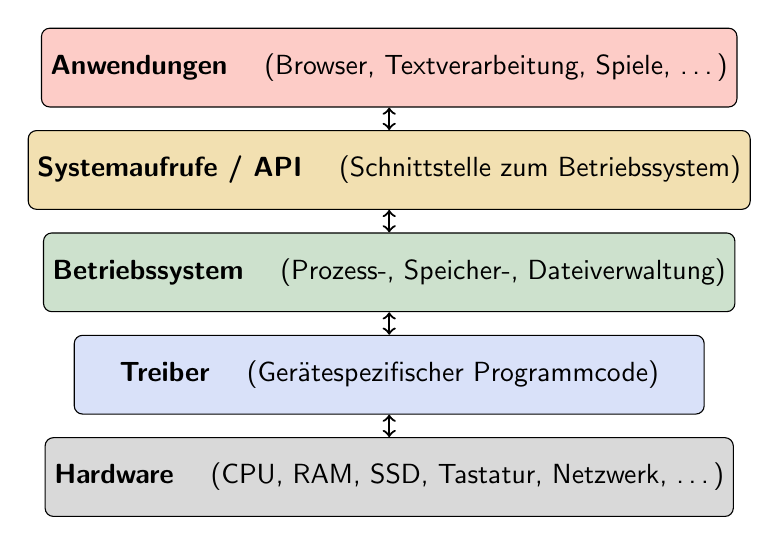
\begin{tikzpicture}[
        layer/.style={draw, minimum width=8cm, minimum height=1cm, text centered, rounded corners=3pt},
        every node/.style={font=\sffamily}
    ]
        \node[layer, fill=Salmon!40]        (app)  at (0, 3.5) {\textbf{Anwendungen} \quad (Browser, Textverarbeitung, Spiele, \ldots)};
        \node[layer, fill=Goldenrod!35]     (api)  at (0, 2.2) {\textbf{Systemaufrufe / API} \quad (Schnittstelle zum Betriebssystem)};
        \node[layer, fill=DarkSeaGreen!45]  (os)   at (0, 0.9) {\textbf{Betriebssystem} \quad (Prozess-, Speicher-, Dateiverwaltung)};
        \node[layer, fill=RoyalBlue!20]     (drv)  at (0,-0.4) {\textbf{Treiber} \quad (Gerätespezifischer Programmcode)};
        \node[layer, fill=Gray!30]          (hw)   at (0,-1.7) {\textbf{Hardware} \quad (CPU, RAM, SSD, Tastatur, Netzwerk, \ldots)};

        \draw[<->, thick] (app)  -- (api);
        \draw[<->, thick] (api)  -- (os);
        \draw[<->, thick] (os)   -- (drv);
        \draw[<->, thick] (drv)  -- (hw);
    \end{tikzpicture}
    \caption{Der Software-Stack: jede Schicht bietet der darüberliegenden Schicht Dienste an und verbirgt die Komplexität der darunter liegenden Schicht.}
    \label{fig:software_stack}
\end{figure}

Jede Schicht \emph{abstrahiert} die Ebene darunter: Eine Anwendung muss nicht wissen, wie eine Festplatte physisch funktioniert -- sie bittet das Betriebssystem einfach darum, eine Datei zu öffnen.

\begin{myremark}[Abstraktion als roter Faden]
    Das Prinzip der Abstraktion ist Ihnen bereits mehrfach begegnet: Ein Byte abstrahiert von einzelnen Bits (\cref{ch:kodierungen}), ein Gatter abstrahiert von einzelnen Transistoren (\cref{ch:logische_gatter}), und der Software-Stack abstrahiert von der konkreten Hardware. Jede Schicht der Informatik baut auf einer einfacheren, darunterliegenden Schicht auf.
\end{myremark}

\section{Aufgaben des Betriebssystems}

Das Betriebssystem (englisch: \emph{operating system}, OS) übernimmt vier zentrale Aufgaben:

\subsection{Prozessverwaltung}

Ein moderner Computer führt viele Programme \emph{scheinbar gleichzeitig} aus (Browser, Musik-Player, Textverarbeitung, \ldots). Da aber oft nur ein physischer Prozessorkern vorhanden ist (oder deutlich weniger als die Anzahl laufender Programme), teilt das Betriebssystem die CPU-Zeit durch raschen Wechsel auf:

\begin{figure}[H]
    \centering
    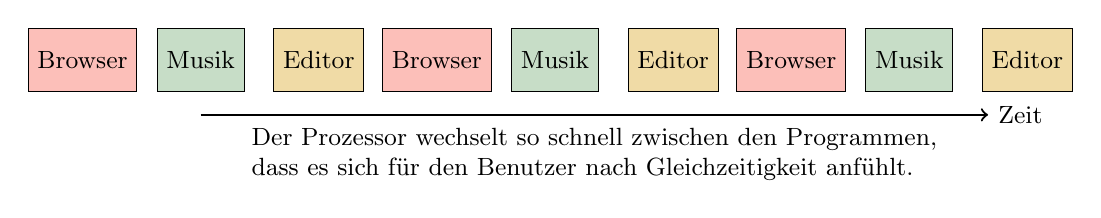
\begin{tikzpicture}[
        proc/.style={draw, fill=RoyalBlue!20, minimum width=2cm, minimum height=0.8cm, text centered, rounded corners},
        time/.style={->, thick},
        every node/.style={font=\small}
    ]
        % Timeline
        \draw[thick, ->] (-0.5,0) -- (9.5,0) node[right] {Zeit};

        % CPU Slots
        \foreach \x/\lbl/\col in {0/Browser/Salmon!50, 1/Musik/DarkSeaGreen!50, 2/Editor/Goldenrod!40, 3/Browser/Salmon!50, 4/Musik/DarkSeaGreen!50, 5/Editor/Goldenrod!40, 6/Browser/Salmon!50, 7/Musik/DarkSeaGreen!50, 8/Editor/Goldenrod!40} {
            \node[draw, fill=\col, minimum width=0.9cm, minimum height=0.8cm, text centered] at (\x*1.5 - 2, 0.7) {\lbl};
        }
        \node[align=left] at (4.5, -0.5) {Der Prozessor wechselt so schnell zwischen den Programmen,\\dass es sich für den Benutzer nach Gleichzeitigkeit anfühlt.};
    \end{tikzpicture}
    \caption{Zeitscheiben-Multitasking: Das Betriebssystem teilt die CPU-Zeit in kleine Scheiben auf.}
    \label{fig:multitasking}
\end{figure}

Ein solcher Zeitabschnitt, der einem Programm zugeteilt wird, heisst \tib{Zeitscheibe}\index{Zeitscheibe} (englisch: \emph{time slice}). Man spricht deshalb auch von \tib{Multitasking}\index{Multitasking}.

\begin{myexercise}
    Ein Prozessorkern teilt seine Rechenzeit auf 5 gleichzeitig laufende Programme auf, wobei jede Zeitscheibe $20\,\mathrm{ms}$ dauert. Nach welcher Zeit ist wieder derselbe Prozess an der Reihe?
    \begin{myanswer}
        $5 \cdot 20\,\mathrm{ms} = 100\,\mathrm{ms}$. Da dies für den Menschen nicht wahrnehmbar ist, wirken die 5 Programme, als würden sie gleichzeitig laufen.
    \end{myanswer}
\end{myexercise}

\subsection{Speicherverwaltung}

Das Betriebssystem weist jedem Prozess einen eigenen Bereich im RAM zu und stellt sicher, dass Prozesse nicht in den Speicherbereich anderer Prozesse eingreifen können (\tib{Speicherschutz}\index{Speicherschutz}). Dies verhindert, dass ein fehlerhaftes oder bösartiges Programm das gesamte System destabilisiert -- vgl. dazu auch die Überlegungen zur Von-Neumann-Architektur in \cref{ch:aufbau_computer}.

\subsection{Dateisystem}

Massenspeicher (SSD, HDD) speichern Daten als rohe Bitsequenzen (vgl. \cref{ch:kodierungen}). Das \tib{Dateisystem}\index{Dateisystem} organisiert diese Bits in \tib{Dateien}\index{Datei} und \tib{Verzeichnisse}\index{Verzeichnis} (Ordner). Es legt fest, wo auf dem Speicher eine Datei beginnt, wie lang sie ist und welche Zugriffsrechte sie hat.

\begin{myexample}[Dateisysteme]
    Bekannte Dateisysteme sind NTFS (Windows), ext4 (Linux) und APFS (macOS). Sie sorgen u.\,a. dafür, dass eine Datei schnell gefunden werden kann und auch nach einem unerwarteten Stromausfall konsistent bleibt.
\end{myexample}

\subsection{Geräteverwaltung und Treiber}

Jedes Peripheriegerät (Drucker, Netzwerkkarte, Grafikkarte, USB-Gerät, \ldots) hat seine eigene Schnittstelle. \tib{Treiber}\index{Treiber} sind kleine Softwaremodule, die dem Betriebssystem mitteilen, wie es mit einem bestimmten Gerät kommunizieren muss. Das Betriebssystem stellt den Anwendungen dann eine einheitliche Schnittstelle bereit -- die Anwendung sendet einfach Druckdaten an das Betriebssystem, ohne sich um Druckermodell oder Treiber zu kümmern.

\section{Zusammenspiel von Hardware, Betriebssystem und Anwendungen}

Um das Zusammenspiel aller Ebenen zu verdeutlichen, verfolgen wir, was passiert, wenn eine Benutzerin die Taste \texttt{A} drückt und das Zeichen im Texteditor erscheint:

\begin{figure}[H]
    \centering
    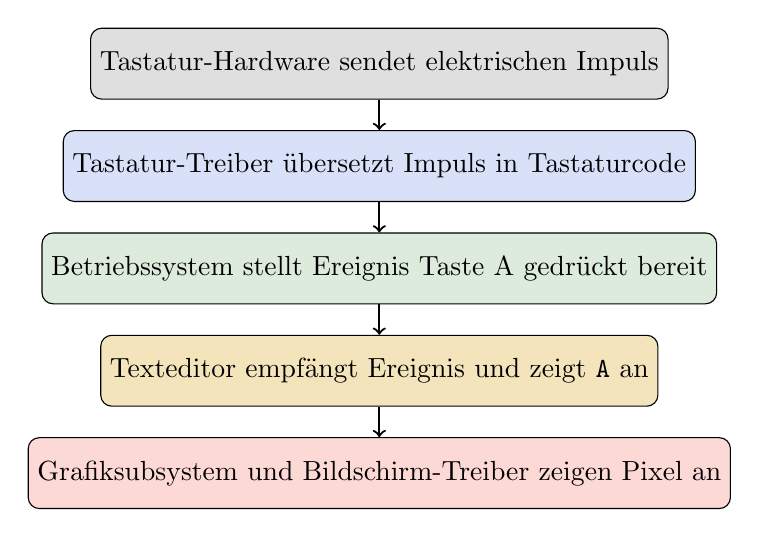
\begin{tikzpicture}[
        stepc/.style={draw, rounded corners, fill=RoyalBlue!15, minimum width=5cm, minimum height=0.9cm, text centered},
        arrow/.style={->, thick}
    ]
        \node[stepc, fill=Gray!25]       (hw)  at (0, 5)   {Tastatur-Hardware sendet elektrischen Impuls};
        \node[stepc, fill=RoyalBlue!20]  (drv) at (0, 3.7) {Tastatur-Treiber übersetzt Impuls in Tastaturcode};
        \node[stepc, fill=DarkSeaGreen!30](os)  at (0, 2.4) {Betriebssystem stellt Ereignis \enquote{Taste A gedrückt} bereit};
        \node[stepc, fill=Goldenrod!30]  (app) at (0, 1.1) {Texteditor empfängt Ereignis und zeigt \texttt{A} an};
        \node[stepc, fill=Salmon!30]     (out) at (0,-0.2) {Grafiksubsystem und Bildschirm-Treiber zeigen Pixel an};

        \draw[arrow] (hw) -- (drv);
        \draw[arrow] (drv) -- (os);
        \draw[arrow] (os) -- (app);
        \draw[arrow] (app) -- (out);
    \end{tikzpicture}
    \caption{Ablauf von Tastendruck bis Bildschirmausgabe -- jede Schicht hat eine klar definierte Aufgabe.}
    \label{fig:tastendruck}
\end{figure}

\begin{myattention}
    Der \enquote{Tastaturcode}, den der Treiber erzeugt, ist letztlich nichts anderes als eine Bitfolge -- ähnlich wie die ASCII-Kodierung aus \cref{ch:kodierungen}, die jedem Zeichen ein Byte zuordnet. Auch die Darstellung des Buchstabens \texttt{A} auf dem Bildschirm läuft letztlich über eine Kodierung von Pixeln und Farben, wie in \cref{ch:kodierungen} besprochen.
\end{myattention}

\begin{myexercise}
    Ordnen Sie die folgenden Komponenten und Aktionen der richtigen Schicht im Software-Stack zu:
    \begin{itemize}
        \item NTFS-Dateisystem
        \item Google Chrome (Browser)
        \item Ein C-Programm ruft \texttt{open("datei.txt")} auf
        \item Der Grafikkartentreiber
        \item Die CPU führt einen Maschinenbefehl aus
    \end{itemize}
    \begin{myanswer}
        \begin{itemize}
            \item NTFS-Dateisystem $\to$ Betriebssystem (Teil des OS-Kernels)
            \item Google Chrome $\to$ Anwendung
            \item \texttt{open("datei.txt")} $\to$ Systemaufruf / API
            \item Grafikkartentreiber $\to$ Treiber
            \item CPU führt Maschinenbefehl aus $\to$ Hardware
        \end{itemize}
    \end{myanswer}
\end{myexercise}

\section{Bekannte Betriebssysteme}

\begin{table}[H]
    \centering
    \begin{tabular}{l|l|l}
        \textbf{Betriebssystem} & \textbf{Hersteller} & \textbf{Typisches Einsatzgebiet} \\\midrule\midrule
        Windows 11              & Microsoft           & PC, Laptop \\\midrule
        macOS                   & Apple               & Mac-Computer \\\midrule
        GNU+Linux (Ubuntu, Debian \ldots) & Open Source  & Server, PC, Laptop, eingebettete Systeme \\\midrule
        Android                 & Google              & Smartphones, Tablets \\\midrule
        iOS                     & Apple               & iPhone, iPad \\
    \end{tabular}
    \caption{Auswahl verbreiteter Betriebssysteme.}
    \label{tab:betriebssysteme}
\end{table}

\begin{myremark}[Open Source]
    Linux ist \tib{Open Source}\index{Open Source}: Der Quellcode des Betriebssystems ist öffentlich einsehbar und kann von jedem verändert und weiterverteilt werden. Dies macht Linux besonders verbreitet im Serverbereich (über 90\,\% der Webserver laufen unter Linux) und in eingebetteten Systemen (Smartphones mit Android, Router, Smart-TVs, \ldots).
\end{myremark}

\begin{mychallenge}
    Sie haben nun den gesamten Weg von der Zahlendarstellung (\cref{ch:zahlendarstellungen}) über Kodierungen (\cref{ch:kodierungen}) und logische Gatter (\cref{ch:logische_gatter}) bis zum vollständigen Computer und Betriebssystem verfolgt. Beschreiben Sie in eigenen Worten, was passiert -- auf allen Ebenen des Software-Stacks --, wenn Sie in einem Texteditor die Tastenkombination \enquote{Strg+S} drücken, um eine Datei zu speichern.
    \begin{myanswer}
        Eine mögliche Antwort: Die Tastatur-Hardware erkennt den Tastendruck und sendet elektrische Impulse, der Tastaturtreiber übersetzt diese in einen Tastaturcode, das Betriebssystem meldet dem Texteditor das Ereignis \enquote{Strg+S gedrückt}. Der Texteditor löst über einen Systemaufruf (API) eine Schreiboperation aus. Das Betriebssystem übersetzt den Text (kodiert z.\,B. als UTF-8-Bitfolge, vgl. \cref{ch:kodierungen}) über das Dateisystem in konkrete Speicherzellen auf der SSD oder HDD und aktualisiert die entsprechenden Metadaten (Dateiname, Grösse, Position). Auf unterster Ebene führt die CPU dabei unzählige Fetch-Decode-Execute-Zyklen (\cref{sec:fde}) aus, die letztlich alle auf einfachen logischen Gattern (\cref{ch:logische_gatter}) beruhen.
    \end{myanswer}
\end{mychallenge}
